\documentclass{beamer}
\setbeamercovered{transparent}
\usepackage{epstopdf}
\usepackage{listings}
\usepackage{lipsum}
\usepackage{subfig}
\usepackage{algorithm}
\usepackage{algorithmicx}
\usepackage{cite}
\usepackage{lipsum}
\usepackage{amssymb}
\usepackage{color}
\usepackage{IEEEtrantools}
\usepackage{booktabs}
\usepackage{texpower}
\usepackage{amsmath}
\usepackage{caption}
\usepackage{multirow}
\usepackage{graphicx}
\newtheorem{Key points}{Key points}
\newtheorem{Summary}{Summary}
\usepackage{dblfloatfix}
%\usepackage{adjustbox}
%\usepackage{animate}
%\usepackage{movie15}
%\usepackage{subfig}
%\newtheorem{Definition}{Definition}
%\usepackage[font={small}]{caption}
\usepackage{beamerthemeshadow}
\newcommand\Fontvi{\fontsize{5}{6.2}\selectfont}
\newcommand\Fontvia{\fontsize{6}{7.2}\selectfont}
\newcommand\Fontviaa{\fontsize{8}{7.2}\selectfont}
\usepackage{listings}
\lstset{language=C++,
                keywordstyle=\color{blue},
                stringstyle=\color{red},
                commentstyle=\color{green},
                morecomment=[l][\color{magenta}]{\#},
                numbers=left,
                escapeinside=||
}

%\captionsetup{font=scriptsize,labelfont=scriptsize}
 \usetheme{Antibes}%PaloAlto
\begin{document}
\title[Lecture 7]{Data Structures and Object Oriented Programming using C++} 
\author[]{Ahsan Ijaz}
\date{}
 \frame{\titlepage}
% \AtBeginSection[]
% {
% \begin{frame}<beamer>{Table of Contents}
% \tableofcontents[currentsection,currentsubsection, 
%     hideothersubsections, 
%     sectionstyle=show/shaded,
% ]
% \end{frame}
% }

 \section{Protected Member}
\frame{\frametitle{Protected Member}
\textbf{Without Inheritance:}
  \begin{itemize}
  \item Same as Private members
  \item Can only be accessed by member functions of class
  \end{itemize}
\textbf{With Public Inheritance:}
\begin{itemize}
\item Private member from base class is {\color{blue}inaccessible} in derived class.
\item Protected member from base class is {\color{blue}accessible} in derived class.
\end{itemize}

 }

 \subsection{Member Access}

 \begin{frame}[fragile]
\frametitle{Member access Error}
\begin{lstlisting}
class Pen {
	public:
		void SetLocation(int, int);
		void SetStatus(int);
	private:
		int x, y, status;};
class ColorPen : public Pen {
	public:
		void SetColor(int);
		void setX(int xx){ x = xx; }//Error! 	
        private:
		int color;
};
\end{lstlisting}
\end{frame}

\begin{frame}[fragile]
\frametitle{Member Can be accessed now}
\begin{lstlisting}
class Pen {
	public:
		void SetLocation(int, int);
		void SetStatus(int);
	protected:
		int x, y;
	private:
		int status;};
class ColorPen : public Pen {
	public:
		void SetColor(int);
		void setX(int xx){ x = xx;}//OK!	
	private:
		int color;
	};
\end{lstlisting}
\end{frame}
\begin{frame}[fragile]
\frametitle{Member Access}
  \begin{figure}
    \centering
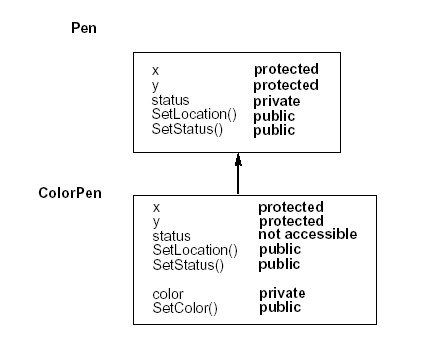
\includegraphics[width=0.8\columnwidth]{protect.png}    
\caption{Protected Member}
  \end{figure}
\end{frame}

\begin{frame}[fragile]
\frametitle{Member Access}
\begin{lstlisting}
void ColorPen::SetColor()
	{x = 1; // error or ok?
	 y = 1; // error or ok?
	 status = 0; // error or ok?
	 color = 2; // error or ok?
	};
void main()
	{ColorPen p;
	 p.x = 1; // error or ok?
	 p.y = 1; // error or ok?
	 p.status = 1; // error or ok?
	 p.color = 1; // error or ok?
	}
\end{lstlisting}
\end{frame}
\begin{frame}[fragile]
\frametitle{Member Access}
\begin{lstlisting}
void ColorPen::SetColor()
	{x = 1; // ok: x is protected in Pen
	 y = 1; // error or ok?
	 status = 0; // error or ok?
	 color = 2; // error or ok?
	};
void main()
	{ColorPen p;
	 p.x = 1; // error or ok?
	 p.y = 1; // error or ok?
	 p.status = 1; // error or ok?
	 p.color = 1; // error or ok?
	}
\end{lstlisting}
\end{frame}
\begin{frame}[fragile]
\frametitle{Member Access}
\begin{lstlisting}
void ColorPen::SetColor()
	{x = 1; // ok: x is protected in Pen
	 y = 1; // ok: y is protected in Pen
	 status = 0; // error or ok?
	 color = 2; // error or ok?
	};
void main()
	{ColorPen p;
	 p.x = 1; // error or ok?
	 p.y = 1; // error or ok?
	 p.status = 1; // error or ok?
	 p.color = 1; // error or ok?
	}
\end{lstlisting}
\end{frame}

\begin{frame}[fragile]
\frametitle{Member Access}
\begin{lstlisting}
void ColorPen::SetColor()
	{x = 1; // ok: x is protected in Pen
	 y = 1; // ok: y is protected in Pen
	 status = 0; // error: status is invisible
	 color = 2; // ok: color is private in Colorpen
	};
void main()
	{ColorPen p;
	 p.x = 1; // error or ok?
	 p.y = 1; // error or ok?
	 p.status = 1; // error or ok?
	 p.color = 1; // error or ok?
	}
\end{lstlisting}
\end{frame}

\frame{\frametitle{Protected Member Summary}

\begin{itemize}
\item Private members from base class are {\color{blue}inaccessible} in derived class.
\item  Protected members from base class are {\color{blue}accessible} to member functions of derived class.
\item Both private and protected members are inaccessible in main() (outside class, both act as private members) and are inaccessible to users.
\end{itemize}
 }
\section{Constructors in Inheritance}
\frame{\frametitle{Object Composition}
  \begin{itemize}
  \item An object of the derived class consists of sub-object of its base classes and the derived class portion.
\item To construct an object of the derived class, objects of the base classes are constructed first.
  \end{itemize}
  \begin{figure}
    \centering
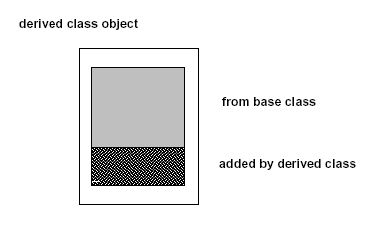
\includegraphics[width=0.6\columnwidth]{comp.png}    
\caption{Composition}
  \end{figure}
}
\begin{frame}[fragile]
\frametitle{Constructors in Multiple inheritance}
\begin{lstlisting}
class Base {
// ...
};

class Derived : public Base{
// ...
};

class DoubleDerived : public Derived {
// ...
};
DoubleDerived dd;
\end{lstlisting}
\end{frame}

\frame{\frametitle{Composition of Multiple Inheritance}
  \begin{figure}
    \centering
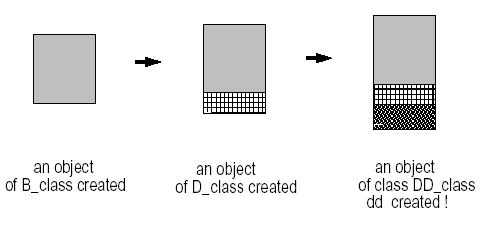
\includegraphics[width=0.8\columnwidth]{mcomp.png}    
\caption{Composition in case of Multiple inheritance}
  \end{figure}
}
\frame{\frametitle{Constructor Call order}
  \begin{itemize}
  \item In an inheritance hierarchy, constructors execute in a \textbf{base class to derived class order.}
  \end{itemize}
\pause
Derived objects are constructed by the following steps:
\begin{itemize}
\item <3-> Allocate space for the entire object( base class members and derived class members)
\item <4-> Invoke the base class constructor to initialize the base class part of the object.
\item <5->Invoke the derived class constructor to initialize the derived class part of the object.
\end{itemize}
}
\begin{frame}[fragile]
\frametitle{Constructor Call Order}
 \begin{columns}[onlytextwidth]
\Fontviaa
     \begin{column}{0.5\textwidth}
       \centering
\begin{lstlisting}
class B_class 
{public:
	B_class(){ cout << "creating Bclass\n";};
};
class D_class : public B_class{
public:
D_class()
{ cout << "constructing Dclass\n"; }
};
int main(){
D_class d; // output?
}
\end{lstlisting}
    \end{column}
\pause
    \begin{column}{0.4\textwidth}
      \centering
      \begin{itemize}
      \item creating Bclass
      \item constructing Dclass
      \end{itemize}
\end{column}
\end{columns}
\end{frame}
\begin{frame}[fragile]
\frametitle{Constructor Calling Example}
\textbf{Consider the following code. What is wrong?}
\begin{lstlisting}
class B_class {
public:
	B_class(int a, int b) : privateA(a), privateB(b) {}
private:
	int privateA, privateB;
};
class D_class : public B_class{
	public:
		D_class( int zz ) : D_privateA(zz) {}
	Private:
		int D_privateA;   
};
int main(){
	D_class d( 10 ); //....
	}
\end{lstlisting}
\end{frame}
\begin{frame}[fragile]
\frametitle{Constructor Calling Example}
\textbf{Solution 1:} Provide a default constructor to the base class.
\Fontviaa
\begin{lstlisting}
class B_class {
	public:
	B_class(int a, int b) : privateA(a), privateB(b) {}
		B_class() {}
	private:
	int privateA, privateB;
	};
class D_class : public B_class{
	public:
		D_class( int zz ) : D_privateA(zz) {}
	private:
		int D_privateA;
	};
int main(){
	D_class d( 10 );
}
\end{lstlisting}
\end{frame}
\begin{frame}[fragile]
\frametitle{Constructor Calling Example}
\textbf{Solution 2:} Explicitly invokes a B class constructor in D class constructor initializer.
\Fontviaa
\begin{lstlisting}
class B_class {
	public:
        B_class(int a, int b) : privateA(a), privateB(b) {}
	private:
	    int privateA, privateB;
	};
class D_class : public B_class{
	public:
        D_class( int zz, int a, int b ) : B_class(a,b), D_privateA(zz){} 
	private:	
	    int D_privateA;
	};
int main(){
	D_class d(10,5,4);
}
\end{lstlisting}
\end{frame}

\subsection{Destructor in Inheritance}
\frame{\frametitle{Destructor}
  \begin{itemize}
  \item When a derived class object is destroyed, the derived class portion is destroyed first.
\item In an inheritance hierarchy, destructors execute in a derived class to base class order, which is the reverse order of constructors.
  \end{itemize}
}
\begin{frame}[fragile]
\frametitle{Destructor Example}
\begin{lstlisting}
class B_class {
	public:
		B_class(){cout<<"Creating B_class\n";}
		~B_class(){cout<<"Destroying B_class\n";}
	};
class D_class : public B_class{
	public:
		D_class(){cout<<"Creating D_class \n"; }
		~D_class(){cout<<"Destroying D_class\n";}
	};
int main()
	{D_class d; // Output?
	}
\end{lstlisting}
\end{frame}

\begin{frame}[fragile]
\frametitle{Destructor Example Output}
  \begin{figure}
    \centering
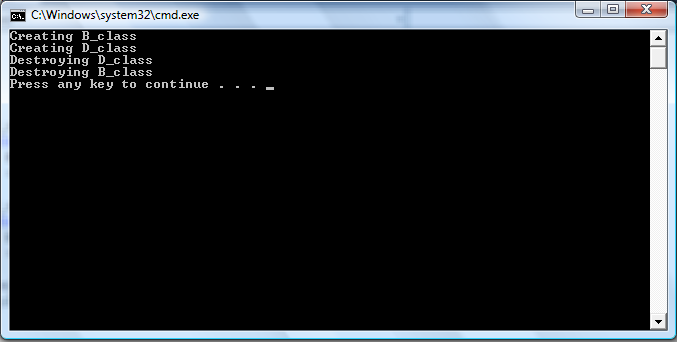
\includegraphics[width=0.8\columnwidth]{des.png}    
\caption{Destructor Output}
  \end{figure}
\end{frame}
\begin{frame}[fragile]
\section{Class Scope and Function Overloading}
\frametitle{Class Scope}
\begin{itemize}
\item Base class members and its derived class members belong to different class scopes.
\item The scope of the derived class can be viewed as nested within the scope of its base class.
\end{itemize}
\end{frame}
\begin{frame}[fragile]
\frametitle{Class Scope}
\begin{lstlisting}
class B_class{
	protected:
		string status;
		int protectedofB;
	private:
		int privateOfB;
	};
class D_class : public B_class{
	public:
		void f();
	private:
		int status;
	};
\end{lstlisting}
\end{frame}
\begin{frame}[fragile]
\frametitle{Class Scope}
\begin{lstlisting}
void D_class::somefunction(){
	status = 1; 
	status = "hello!"; 
	B_class::status = "hello!"; 
	protectedofB = 1; 
	privateOfB = 1; 
}
\end{lstlisting}
\end{frame}

\begin{frame}[fragile]
\frametitle{Class Scope}
\begin{lstlisting}
void D_class::somefunction(){
	status = 1; //Ok
	status = "hello!"; 
	B_class::status = "hello!"; 
	protectedofB = 1; 
	privateOfB = 1; 
}
\end{lstlisting}
\end{frame}

\begin{frame}[fragile]
\frametitle{Class Scope}
\begin{lstlisting}
void D_class::somefunction(){
	status = 1; //Ok
	status = "hello!"; 
//Error, status is resolved to D_class::x
	B_class::status = "hello!"; 
protectedofB = 1; 
	privateOfB = 1; 
}
\end{lstlisting}
\end{frame}

\begin{frame}[fragile]
\frametitle{Class Scope}
\begin{lstlisting}
void D_class::somefunction(){
	status = 1; //Ok
	status = "hello!"; 
//Error, status is resolved to D_class::x
	B_class::status = "hello!";  //Okay
	protectedofB = 1;  
	privateOfB = 1; 
}
\end{lstlisting}
\end{frame}

\begin{frame}[fragile]
\frametitle{Class Scope}
\begin{lstlisting}
void D_class::somefunction(){
	status = 1; //Ok
	status = "hello!"; 
//Error, status is resolved to D_class::x
	B_class::status = "hello!";  //Okay
	protectedofB = 1;  //Okay
	privateOfB = 1; 
}
\end{lstlisting}
\end{frame}

\begin{frame}[fragile]
\frametitle{Class Scope}
\begin{lstlisting}
void D_class::somefunction(){
	status = 1; //Ok
	status = "hello!"; 
//Error, status is resolved to D_class::x
	B_class::status = "hello!";  //Okay
	protectedofB = 1;  //Okay
	privateOfB = 1; 
/*Error, accessing private of Class_B in 
Derived Class*/
}
\end{lstlisting}
\end{frame}
\begin{frame}[fragile]
\frametitle{Function Overloading}
If the derived class adds a member with the {\color{blue}same} name of a member in the base class, the local member {\color{blue}hides} the inherited member.
\end{frame}
\begin{frame}[fragile]
\frametitle{Overloaded Function...Not}
\begin{lstlisting}
class B_class{
	public:
		void overfunction(){ /*...*/ }
	};
class D_class : public B_class{
	public:
		void overfunction(int){ /*...*/ }
	};
int main(){
	D_class x;
	x.overfunction(); //Error
	}
\end{lstlisting}
\end{frame}
\begin{frame}[fragile]
\frametitle{How to overloaded Function}
Qualify the base class member with the class scope operator so it become visible in the derived class scope, and therefore the same named functions can be overloaded.
\end{frame}
\begin{frame}[fragile]
\frametitle{How to overloaded function}
\begin{lstlisting}
class Base{
	public:
		void f(double);
	};
class Derived : public Base{
	public:
		using Base::f;
		void f(int);
	};
\end{lstlisting}
\end{frame}

\section{Type of Inheritance}
\begin{frame}[fragile]
\frametitle{Type of Inheritance}
Class derivation has three types:
\begin{itemize}
\item Public 
\item Private
\item Protected
\end{itemize}
\end{frame}
\begin{frame}[fragile]
\frametitle{Type of Inheritance}
\begin{lstlisting}
class Base{
	//...
	};
// protected inheritance
class Derived1 : protected Base{
	//...
	};
// private inheritance
class Derived2 : Base{ // Caution:
	//...       // inheritance is PRIVATE
	};         // by default !!!
\end{lstlisting}
\end{frame}
% \begin{frame}[fragile]
% \frametitle{Public Inheritance Summary}
% Summary of Public Inheritance:
% \begin{table}[htpb] \centering
% \begin{tabular}{lccc} \toprule
% Accessibility from & Private  & Public & Protected\\\midrule 
% Own Class & Yes & Yes & Yes\\
% Derived Class & No & Yes & Yes\\
% Outside Derived Class & No & Yes  & No\\
% \bottomrule
% \end{tabular}
% \caption{Public Inheritance}
% \end{table}
% \end{frame}
% \begin{frame}[fragile]
% \frametitle{Protected Inheritance Summary}
% Summary of Protected Inheritance:
% \begin{table}[htpb] \centering
% \begin{tabular}{lccc} \toprule
% Accessibility from & Private  & Public & Protected\\\midrule 
% Own Class & Yes & Yes & Yes\\
% Derived Class & No & Yes & Yes\\
% Outside Derived Class & No & Yes  & No\\
% \bottomrule
% \end{tabular}
% \caption{Protected Inheritance}
% \end{table}
% \end{frame}
% \begin{frame}[fragile]
% \frametitle{Private Inheritance Summary}
% Summary of Private Inheritance:
% \begin{table}[htpb] \centering
% \begin{tabular}{lccc} \toprule
% Accessibility from & Private  & Public & Protected\\\midrule 
% Own Class & Yes & Yes & Yes\\
% Derived Class & No & Yes & Yes\\
% Outside Derived Class & No & Yes  & No\\
% \bottomrule
% \end{tabular}
% \caption{Private Inheritance}
% \end{table}
% \end{frame}
\begin{frame}[fragile]
\frametitle{Type and Implementation inheritance}
\begin{itemize}
\item Public derivation is called type inheritance.
\item Private derivation is called implementation inheritance.
\end{itemize}
\end{frame}
\begin{frame}[fragile]
\frametitle{Type of Inheritance}
\Fontvi
\begin{lstlisting}
class A 
{
public:
    int x;
protected:
    int y;
private:
    int z;
};

class B : public A
{
    // x is public
    // y is protected
    // z is not accessible from B
};

class C : protected A
{
    // x is protected
    // y is protected
    // z is not accessible from C
};

class D : private A
{
    // x is private
    // y is private
    // z is not accessible from D
};
\end{lstlisting}
\end{frame}
\end{document}